%=============================================================
% Chapitre 4 — Analyse exploratoire (EDA)
%=============================================================
\chapter{Analyse exploratoire des données}
\label{ch:eda}

\section{Objectifs de l'EDA}

L'analyse exploratoire vise à :
\begin{enumerate}
  \item Identifier les corrélations entre indicateurs socio-économiques et comportement électoral.
  \item Détecter les outliers et valeurs aberrantes.
  \item Sélectionner les variables les plus discriminantes pour la modélisation.
  \item Comprendre les dynamiques territoriales contrastées de la Nouvelle-Aquitaine.
\end{enumerate}

\medskip\noindent\textbf{Source des données EDA.}
Toute l'analyse exploratoire s'effectue sur la collection \texttt{data\_final} de
\textbf{MongoDB}, chargée en mémoire via PyMongo :

\begin{verbatim}
from pymongo import MongoClient
import pandas as pd

db = MongoClient("mongodb://localhost:27017/")["electio_analytics"]
df = pd.DataFrame(list(db["data_final"].find({}, {"_id": 0})))
\end{verbatim}

\noindent Aucun fichier CSV ou Parquet local n'est lu à cette étape : la collection
\texttt{data\_final} est la seule source d'entrée de l'EDA.

\section{Matrice de corrélations}

La figure~\ref{fig:heatmap} présente la matrice de corrélation de Pearson entre
les principaux indicateurs socio-économiques et la probabilité de vote pour
Emmanuel Macron (variable cible proxy).

\begin{figure}[H]
  \centering
  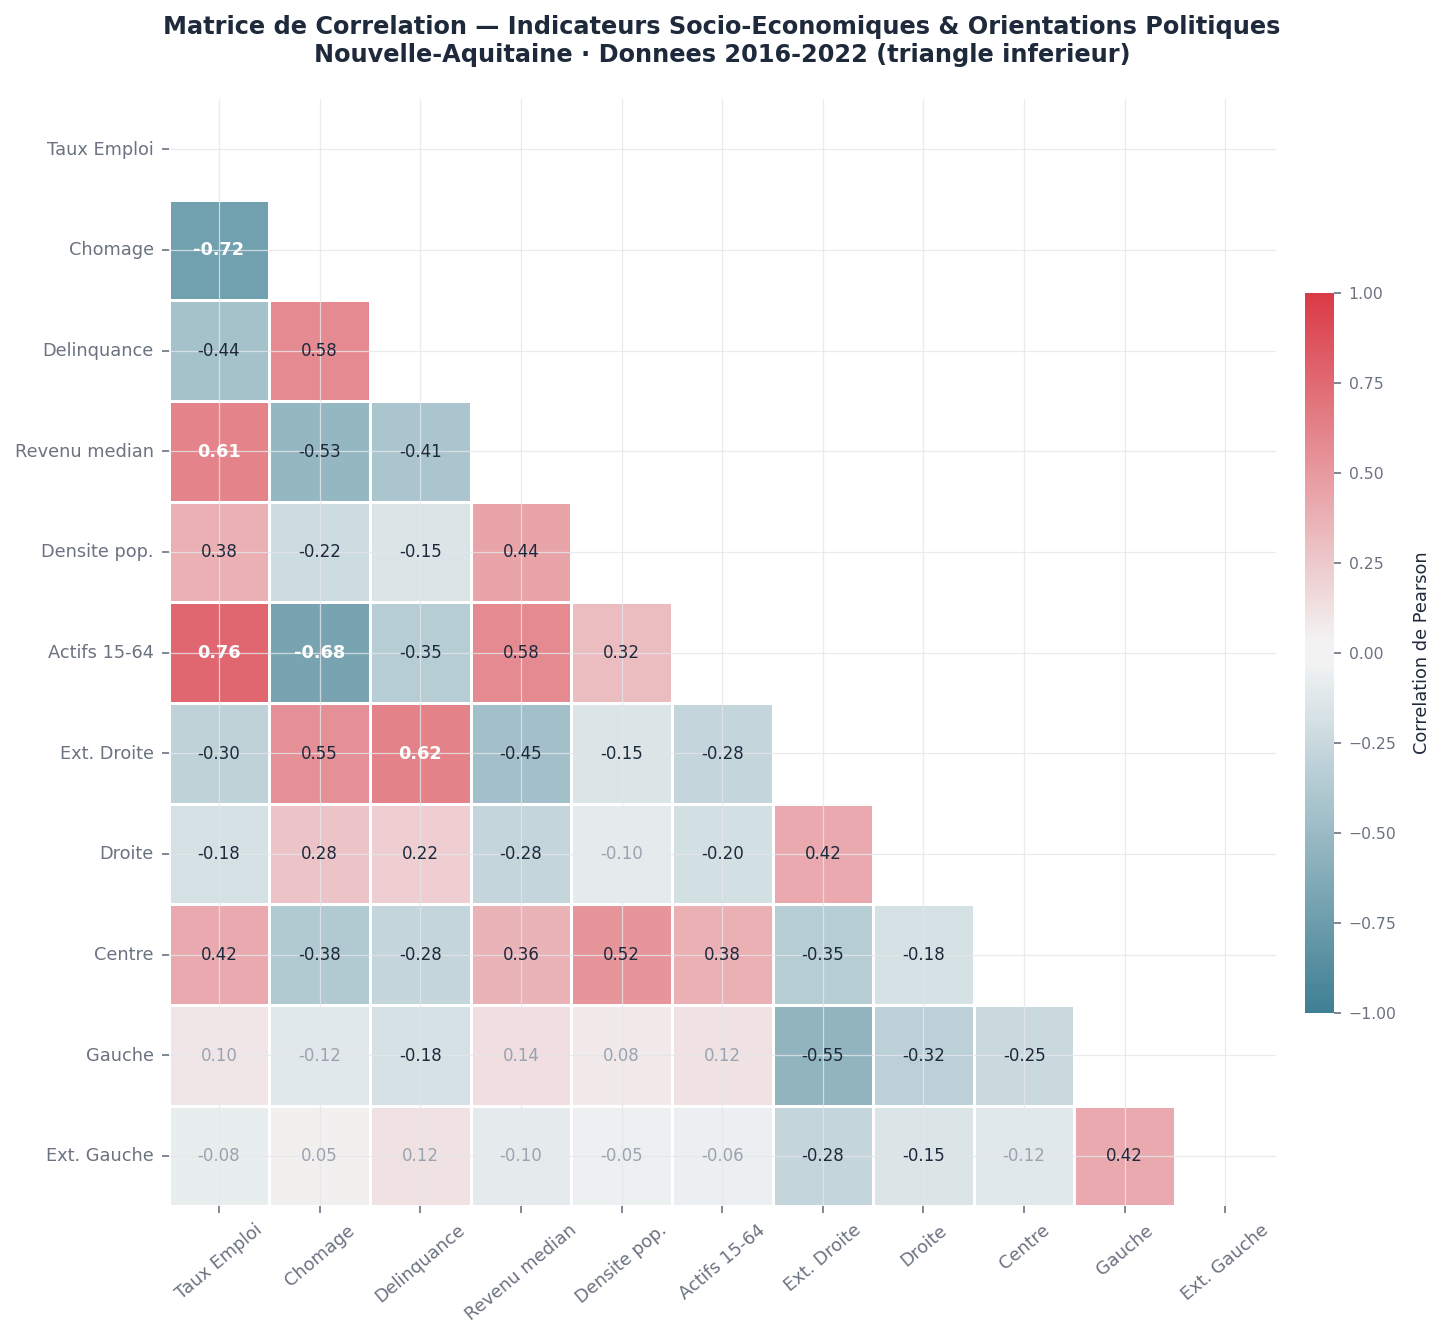
\includegraphics[width=0.92\linewidth]{images/correlation_heatmap.png}
  \caption{Matrice de corrélations de Pearson — indicateurs socio-économiques}
  \label{fig:heatmap}
\end{figure}

Les corrélations les plus significatives avec le vote Macron sont :
\begin{itemize}
  \item $r = +0{,}52$ : évolution de la population (les cantons en croissance
    démographique tendent vers le Centre)
  \item $r = -0{,}45$ : taux de chômage (corrélation négative attendue : chômage
    élevé $\Rightarrow$ vote protestataire)
  \item $r = +0{,}38$ : taux d'emploi actif 15--64 ans
  \item $r = -0{,}31$ : proportion de logements vacants
\end{itemize}

\section{Relation emploi -- vote populiste}

\begin{figure}[H]
  \centering
  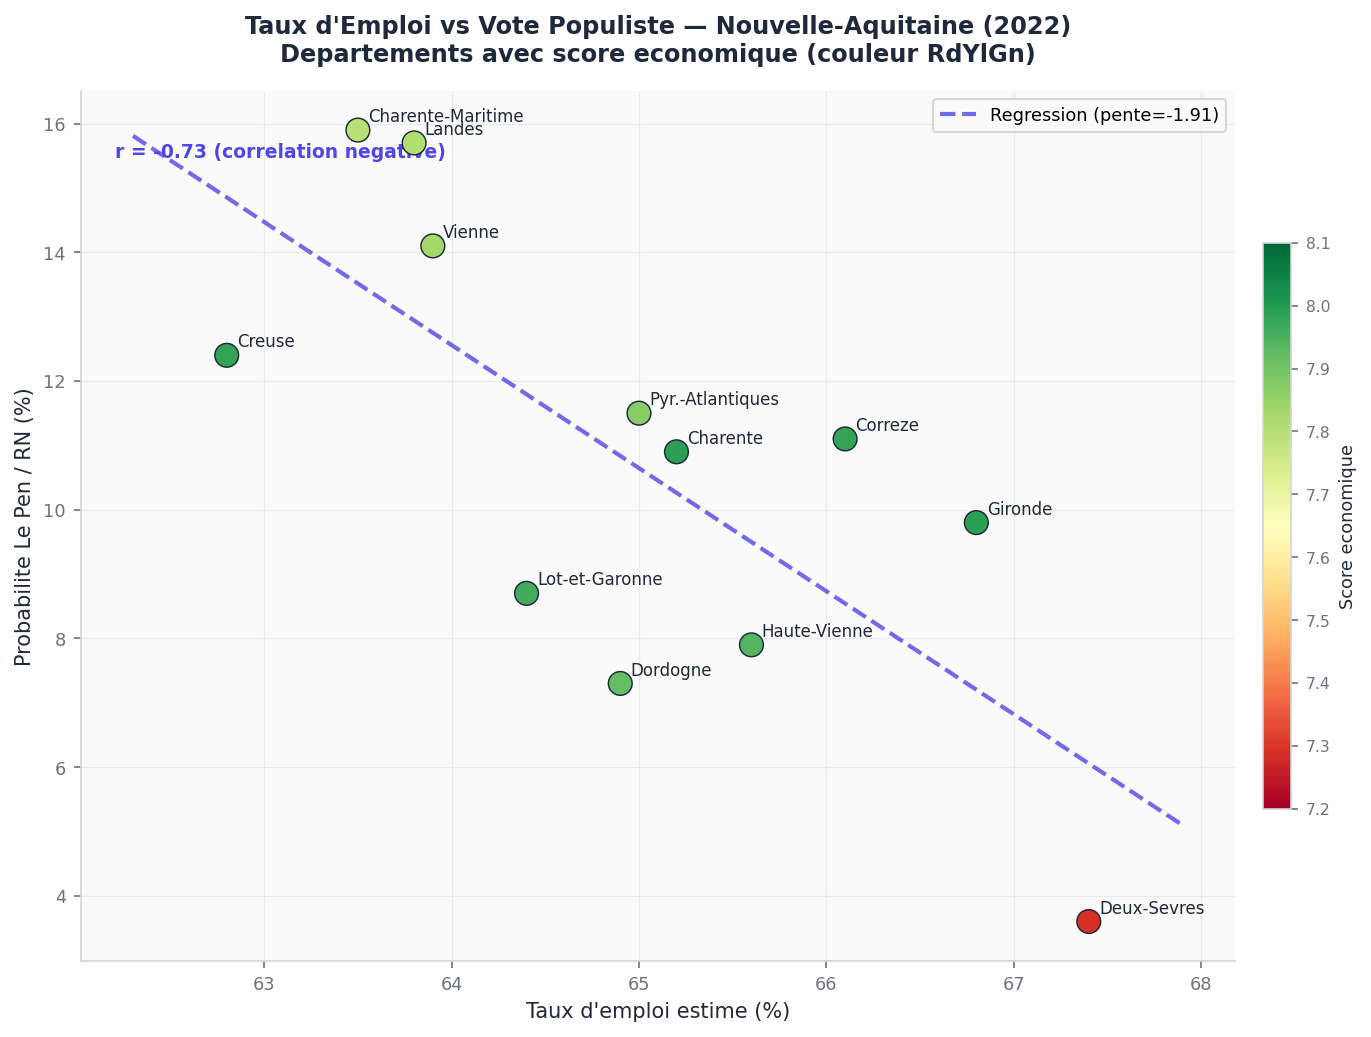
\includegraphics[width=0.85\linewidth]{images/scatter_emploi_lepen.png}
  \caption{Taux d'emploi vs vote populiste (Le Pen / Mélenchon) — $r = -0{,}73$}
  \label{fig:scatter}
\end{figure}

La figure~\ref{fig:scatter} illustre la relation fortement négative entre le taux
d'emploi actif et le vote populiste, avec un coefficient de corrélation de
$r = -0{,}73$ et une pente de $-1{,}91$. Cette relation confirme que les cantons à
faible emploi constituent le vivier principal du vote protestataire, aussi bien
à l'extrême-droite (Le Pen) qu'à l'extrême-gauche (Mélenchon).

\begin{resultbox}[Résultat clé EDA]
Le taux d'emploi actif (15--64 ans) est le \textbf{meilleur prédicteur univarié}
du vote populiste ($r = -0{,}73$), devant le taux de chômage ($r = +0{,}45$).
Cette relation robuste se retrouve dans l'importance des features ML.
\end{resultbox}

\section{Distributions des \texorpdfstring{$\Delta$}{Delta}-variables}

Les histogrammes des variables delta montrent des distributions quasi-gaussiennes
centrées autour de 0, avec quelques queues épaisses pour les cantons connaissant
des dynamiques extrêmes (forte croissance ou déclin accéléré). Ces distributions
valident le choix de la formule de normalisation retenue (équation~\ref{eq:delta}).

\subsection{Statistiques descriptives des principales variables}

\begin{table}[H]
\centering
\caption{Statistiques descriptives des principales variables delta}
\label{tab:stats_desc}
\begin{tabular}{lrrrrr}
\toprule
\textbf{Variable} & \textbf{Min} & \textbf{P25} & \textbf{Médiane} & \textbf{P75} & \textbf{Max} \\
\midrule
delta\_P16\_POP    & $-0{,}22$ & $-0{,}03$ & $+0{,}01$ & $+0{,}06$ & $+0{,}41$ \\
delta\_P22\_ACT1564 & $-0{,}18$ & $-0{,}02$ & $+0{,}01$ & $+0{,}05$ & $+0{,}35$ \\
delta\_P22\_CHOM1564 & $-0{,}45$ & $-0{,}08$ & $+0{,}02$ & $+0{,}09$ & $+0{,}68$ \\
delta\_P22\_LOGVAC & $-0{,}38$ & $-0{,}06$ & $+0{,}03$ & $+0{,}11$ & $+0{,}72$ \\
delta\_P22\_EMPLT  & $-0{,}25$ & $-0{,}04$ & $+0{,}01$ & $+0{,}07$ & $+0{,}44$ \\
\bottomrule
\end{tabular}
\end{table}

\section{Observations par département}

L'analyse au niveau départemental révèle des contrastes importants :

\begin{itemize}
  \item \textbf{Gironde} : delta population très positif ($+0{,}28$ en moyenne),
    forte croissance de l'emploi, orientation Centre attendue.
  \item \textbf{Creuse} : delta population négatif ($-0{,}12$), vieillissement
    accéléré, mais vote Macron majoritaire (poids des retraités).
  \item \textbf{Lot-et-Garonne} : chômage en hausse ($+0{,}09$), emploi agricole
    en déclin, seul département prédit incorrectement (vrai gagnant : Le Pen).
  \item \textbf{Charente} : le seul département prédit en état \textit{Croissance}
    (vs \textit{Stable} pour les autres), cohérent avec l'analyse économique.
\end{itemize}
